%----------------------------------------------------------------------------------------
%    PACKAGES AND THEMES
%----------------------------------------------------------------------------------------

\documentclass[aspectratio=169,xcolor=dvipsnames]{beamer}
\usetheme{SimpleDarkBlue}
\usepackage{tikz}
\usetikzlibrary{arrows.meta,decorations.pathmorphing,positioning}
\usepackage{graphicx}
\usepackage{pdfpages}
\usepackage{graphicx} % Allows including images
\usepackage{booktabs} % Allows the use of \toprule, \midrule and \bottomrule in tables
\usepackage{hyperref}
%----------------------------------------------------------------------------------------
%    TITLE PAGE
%----------------------------------------------------------------------------------------

\title{Knowledge Distillation Using Early Exit LLMs}
\subtitle{Experiments on Confidence Scoring}

\author{ Edvin 24V0074 \and Sagar 24D0367 }
% Kapil 210100079 }

\institute
{
    CS 769 \\
    Optimization in Machine Learning % Your institution for the title page
}
\date{20 March 2016} % Date, can be changed to a custom date

%----------------------------------------------------------------------------------------
%    PRESENTATION SLIDES
%----------------------------------------------------------------------------------------

\begin{document}

\begin{frame}
    % Print the title page as the first slide
    \titlepage
\end{frame}

\begin{frame}{Overview}
    % Throughout your presentation, if you choose to use \section{} and \subsection{} commands, these will automatically be printed on this slide as an overview of your presentation
    \tableofcontents
\end{frame}


\section{Knowledge Distillation}

\begin{frame}<1-4>[label=slide:KD]{Knowledge Distillation}
    \begin{columns}
        \begin{column}{0.4\textwidth}
            \begin{itemize}
                \item<1-> Introduced in \cite{hinton_distilling_2015} % 
                \item<2-> Student - teacher models 
                \item<3-> Teacher Provides "Soft Targets"
                \item<4-> Loss: kl divergence $+$ cross-entropy
                \item<5-> Training Specialist Models 
            \end{itemize}
        \end{column}

        \begin{column}{0.6\textwidth}
            \only<1>{Large Cumbersome Models are difficult to deploy need to train smaller models efficiently}
            \only<2>{Smaller Student model tries to mimic larger teacher model that generalises well \\
            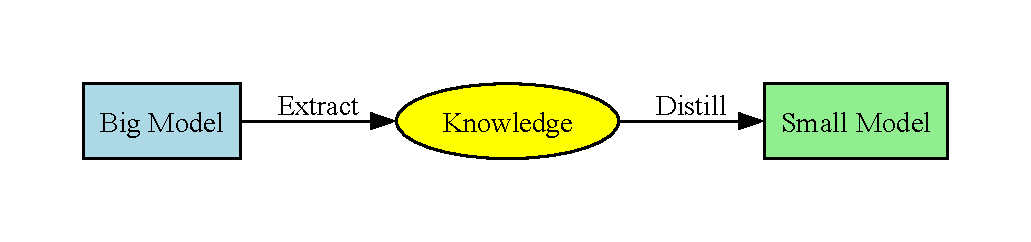
\includegraphics[width=\textwidth]{test.pdf}}
            \only<3>{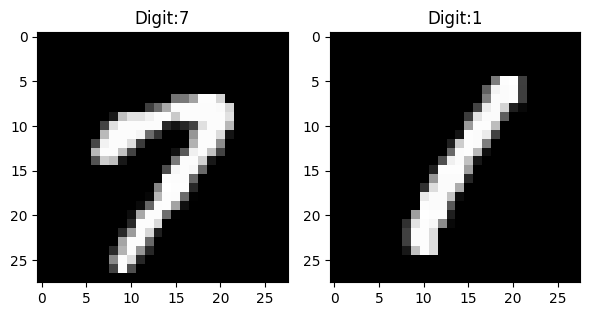
\includegraphics[width=\textwidth]{figs/MNIST.png} \\
            \[ q_i = \frac{exp(z_i / T)}{\sum_j exp(z_i/T)} \]}
            \only<4>{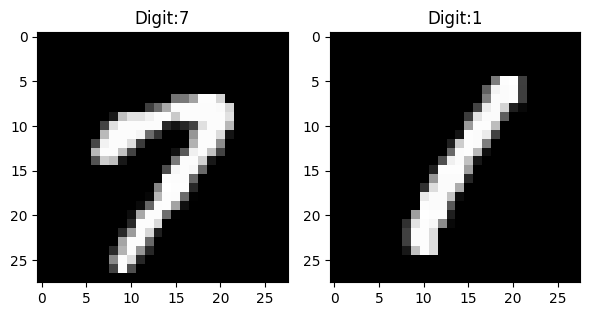
\includegraphics[width=0.6\textwidth]{figs/MNIST.png}
                    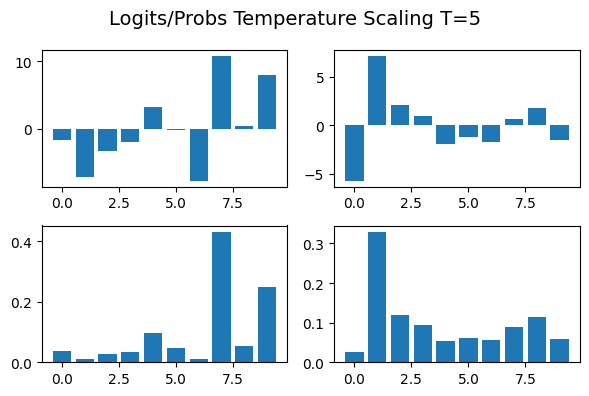
\includegraphics[width=0.6\textwidth]{figs/Logits.png}
            }
        \end{column}
    \end{columns}
    
\end{frame}

% \againframe<3-4>{slide:KD}
% \item<2-> Smaller Student model that mimics larger teacher model that generalises well
% \item<3-> The negative examples give info about dataset that is not captured by the cross entropy loss
% \item<4-> Teacher Provides "Soft Targets"
% \item<5-> minimise the kl divergence of last layer logits of the teacher along with cross entropy loss
% \begin{tikzpicture}<1>
%     \node at (0,0){Text Test};
% \end{tikzpicture}

\section{KD with early exits}
\begin{frame}{KD with early exits}
    \begin{columns}
        \begin{column}{0.4\textwidth}
            \begin{itemize}
                \item<1-> Proposed by \cite{tiwari_using_2024} % 
                \item<2-> Student model relies on spurious correlations
                \item<3-> Student's early Layers overconfident on hard instances
                \item<4-> DEDIER training
                \item<5-> Experiments
            \end{itemize}
        \end{column}

        \begin{column}{0.6\textwidth}
            \only<2>{Smaller Models trained via KD rely more on spurious correlations than the teacher model, which 
            leads to Poor performance on group fairness metrics by the student \\
            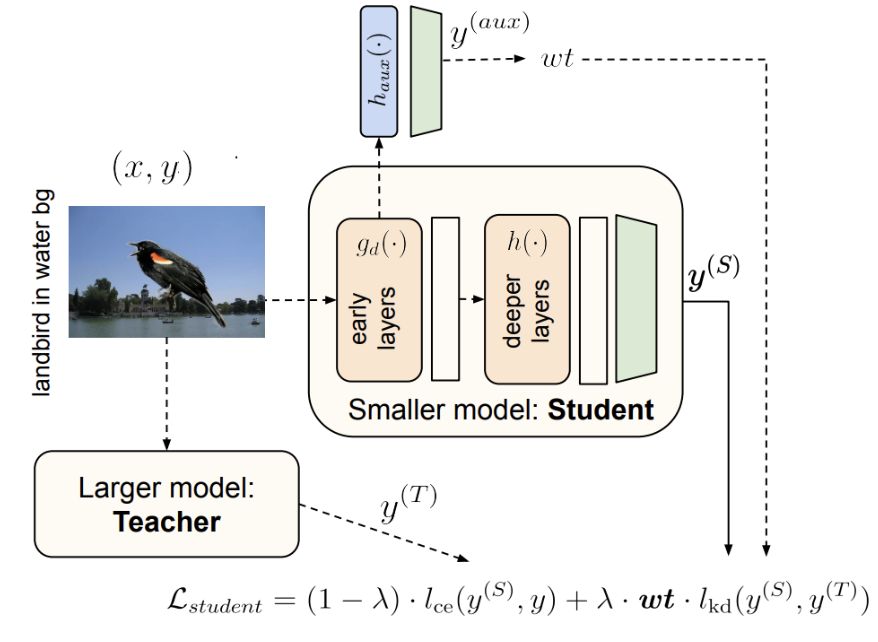
\includegraphics[width=\textwidth]{figs/fig_4.png}}
            \only<3>{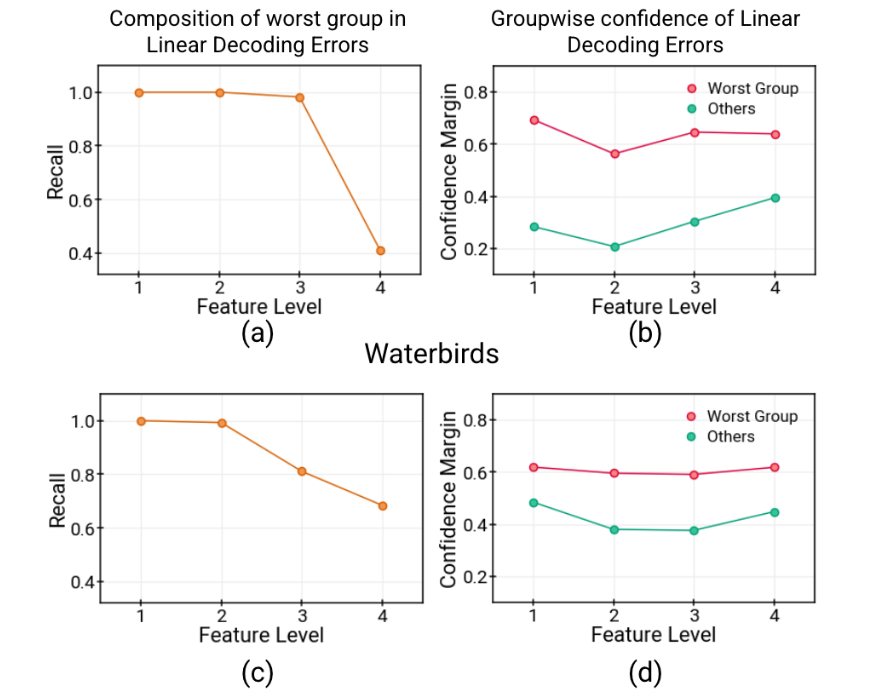
\includegraphics[width=\textwidth]{figs/fig_5.png}}
            \only<4>{
                \[ \mathcal{L}_{student} =
          \sum_{D_w}^{} (1- \lambda) \cdot l_{ce} 
          + \lambda \cdot \textbf{wt} \cdot l_{ke} \] 
          where \(\bf{wt} = \exp^{\beta.\bf{cm}.\alpha} \) }
            \only<5>{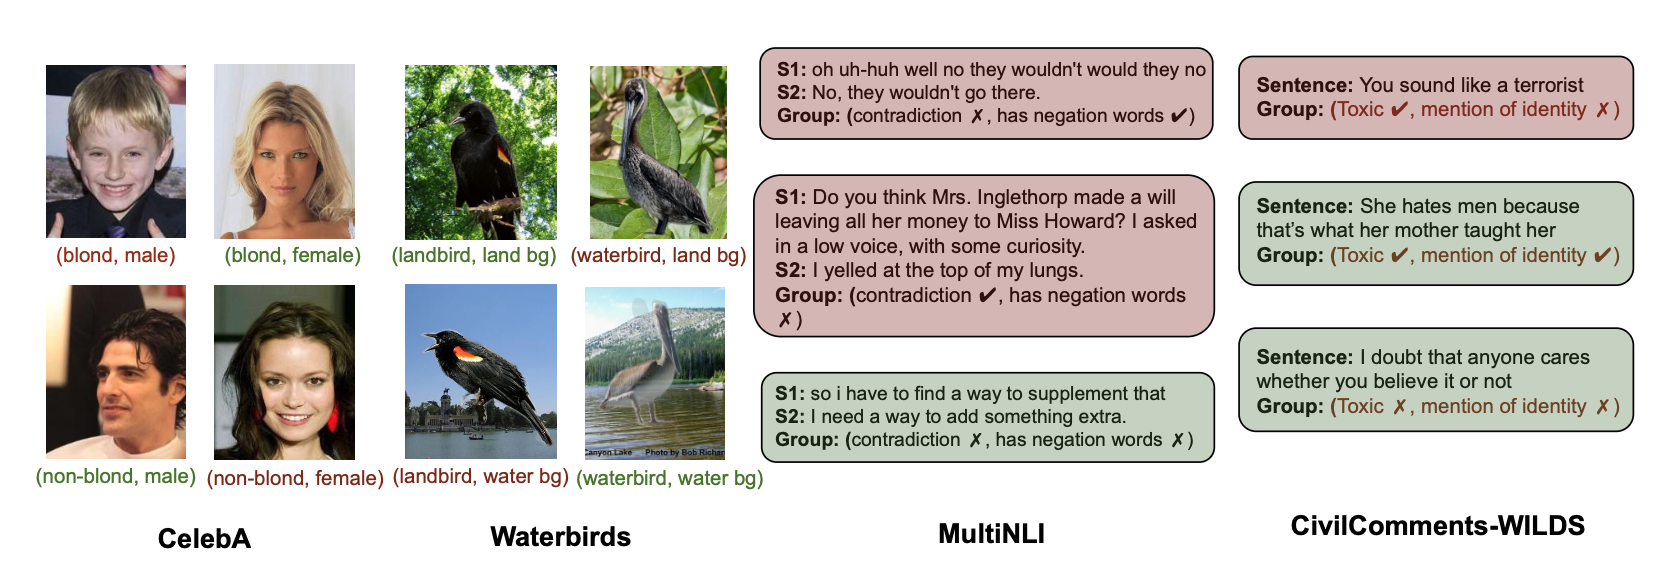
\includegraphics[width=\textwidth]{figs/fig_6.png}}
            \only<6>{Compared to some other methods \\
                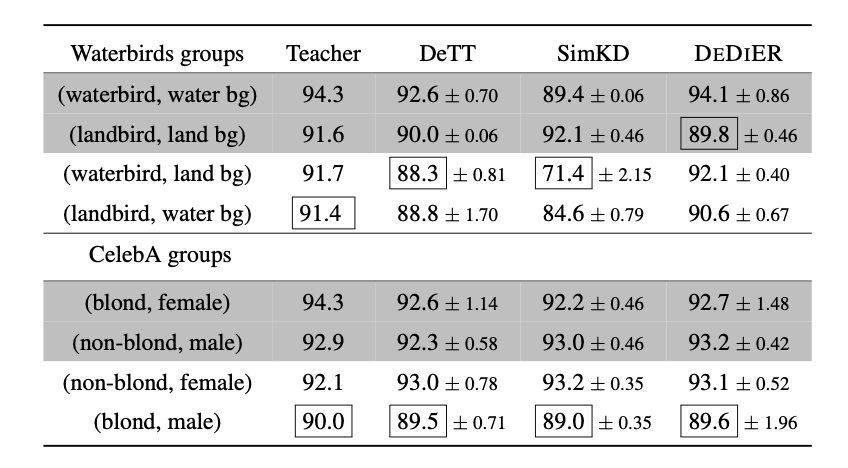
\includegraphics[width=0.6\textwidth]{figs/fig_7.png} \\ 
                Adaptive to the dataset \\
                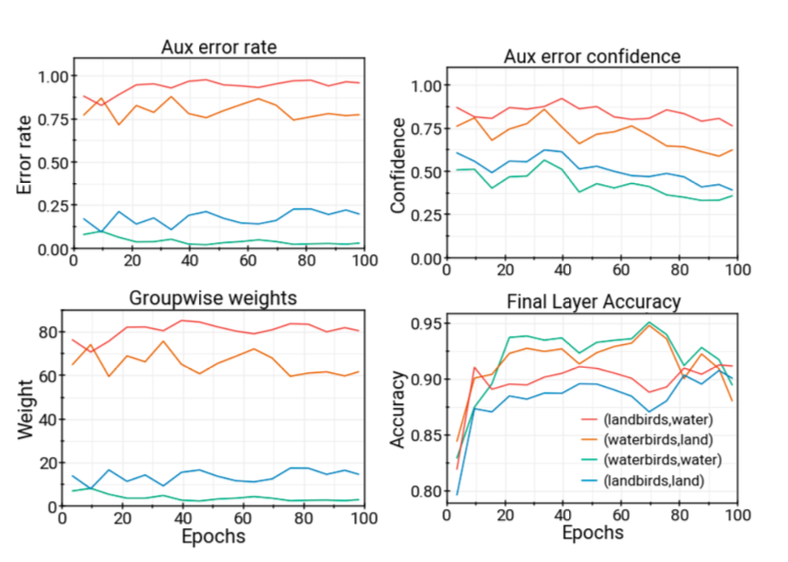
\includegraphics[width=0.6\textwidth]{figs/fig_8.png}}
        \end{column}
    \end{columns}
    
\end{frame}

\section{Early-Exit with Nested Prediction Sets}

\begin{frame}{Early-Exit with Nested Prediction Sets}

    \begin{columns}
        \begin{column}{0.4\textwidth}
            \begin{itemize}
                \item<1-> \cite{jazbec_early-exit_2024} \textbf{A}nytime\textbf{V}alid\textbf{C}onfidence\textbf{S}equences(AVCS) % 
                \item<2-> AVCS has time uniform and non - asymptotic guarantees
                \item<3-> Martingales And Ville's theorem
                \item<4-> Predictive-likelihood ratio
                \item<5-> AVCS for Regression
                \item<6-> AVCS for Classification
                \item<7-> Post-Hoc Implementation
            \end{itemize}
        \end{column}

        \begin{column}{0.6\textwidth}
            \only<1>{\cite{jazbec_early-exit_2024} propose using \textbf{A}nytime\textbf{V}alid\textbf{C}onfidence
            \textbf{S}equences(AVCS) for uncertainity estimation in Early Exit Networks}
            \only<2>{ \[\mathcal{C}_t = (l_t, r_t) \subseteq \mathbb{R} \]
             \[\mathcal{L}(W_{1:T}, U_{1:T}; \mathcal{D}) = \sum_{n=1}^{N} \frac{1}{T} \sum_{t=1}^{T} \ell(y_n, f(x_n; W_t, U_{1:t}))
            \]
            \[\text{size}(t) := \frac{1}{n_{\text{test}}} \sum_{n=1}^{n_{\text{test}}} |\mathcal{C}_t(x_n)|
    \]
           \[\text{coverage}(t) := \frac{1}{n_{\text{test}}} \sum_{n=1}^{n_{\text{test}}} \left[ y_n \in \mathcal{C}_t(x_n) \right]
    \]
    \[\mathcal{N}(t) = |\bigcap_{s \leq t} \mathcal{C}_s| / |\mathcal{C}_t| \]
            \[\mathbb{P}(\forall t,\, \theta^* \in \mathcal{C}_t) \geq 1 - \alpha
    \] 
    } %  Interval notation, 
            
            \only<3>{\[\mathbb{E}_{x_{t+1}} \left[ R_{t+1}(\theta^*) \,\middle|\, x_1, \ldots, x_t \right] = R_t(\theta^*)
            \]
            \begin{displaymath}
                \mathbb{P}(\exists t : R_t(\theta^*) \geq 1/\alpha) \leq \alpha
            \end{displaymath}

            \[\mathcal{C}_t := \{\theta : R_t(\theta) \leq 1/\alpha \} \] } % Confidence set definition
            
            \only<4>{Idea is to create a sequence of martingales for each exit layer and then
    use Ville's theorem to construct AVCS. \\
    \[ R_t^*(y) = \prod_{l=1}^{t} \frac{p_l(y| x^*, \mathcal{D})}
        {p(y| x^*, W_l)} , W_l \sim p(W_l | D^* )\]}
            
            \only<5>{\begin{gather*} % posterior and predictive dsitribution
                y \sim \mathcal{N}\left(y; h_t(x)^T W_t, \sigma_t^2\right), \\
                W_t \sim \mathcal{N}(W_t; \hat{W}_t, \sigma_{w,t}^2 \mathbb{I}_H) \\
                p(W_t | \mathcal{D}) = \mathcal{N}(W_t; \mu_t, \Sigma_t), \quad \\ 
                p_t(y | x^*, \mathcal{D}) = \mathcal{N}(y; h_t(x^*)^T \mu_t, v_* + \sigma_t^2)
            \end{gather*} 
            }
            
            \only<6>{\begin{gather*} % posterior and predictive dsitribution classification
                p(y | \pi_t) = \text{Cat}(y | \pi_t), \\
                p(\pi_t | x^*, \mathcal{D}) = \text{Dir}(\pi_t | \alpha_t(x^*; \mathcal{D})) \\ 
                p_t(y = y | x^*, \mathcal{D}) = \int p(y = y | \pi_t) \, p(\pi_t | x^*, \mathcal{D}) \, d\pi_t  \\
                = \frac{\alpha_{t,y}}{\sum_{y' \in \mathcal{Y}} \alpha_{t,y'}}
            \end{gather*} 
            }

            \only<7>{\[ a_t(x) = \text{ReLU}(x, \tau_t) \]}
        \end{column}
    \end{columns}
\end{frame}


\begin{frame}{Evaluations}
    \begin{columns} % T aliign top
        \column{0.5\textwidth}
        \begin{gather*}
            \mathcal{C}_t = (l_t, r_t) \subseteq \mathbb{R} \\
            \mathcal{L}(W_{1:T}, U_{1:T}; \mathcal{D}) =  \\
            \sum_{n=1}^{N} \frac{1}{T} \sum_{t=1}^{T} \ell(y_n, f(x_n; W_t, U_{1:t})) \\
            \text{size}(t) := \frac{1}{n_{\text{test}}} \sum_{n=1}^{n_{\text{test}}} |\mathcal{C}_t(x_n)| \\ 
            \text{coverage}(t) := \frac{1}{n_{\text{test}}} \sum_{n=1}^{n_{\text{test}}} \left[ y_n \in \mathcal{C}_t(x_n) \right] \\
            \mathcal{N}(t) = |\bigcap_{s \leq t} \mathcal{C}_s| / |\mathcal{C}_t| \\
            \mathbb{P}(\forall t,\, \theta^* \in \mathcal{C}_t) \geq 1 - \alpha 
        \end{gather*}
        
        \column{0.5\textwidth}
        \includegraphics<1>[width=0.6\textwidth]{figs/fig_2.png}
        \includegraphics<2>[width=\textwidth]{figs/fig_1.png}
        \includegraphics<3>[width=\textwidth]{figs/fig_3.png}
        
    \end{columns}
\end{frame}


\section{Fixing overconfidence in Dynamic Neural Networks}
\begin{frame}{Fixing overconfidence in Dynamic Neural Networks}
    % \textit{IEEE/CVF Winter Conference on Applications of Computer Vision (WACV) 2024
    % }
\cite{meronen_fixing_2023}
    \begin{itemize}
        \item To decrease computational cost, we do not want to run network for more layers that required for the specific task
        \item To be able to know where to stop, the model needs good uncertainty estimates
        \item The paper aims to improve uncertainty estimates for a model
    \end{itemize}
    \begin{figure}
        \centering
        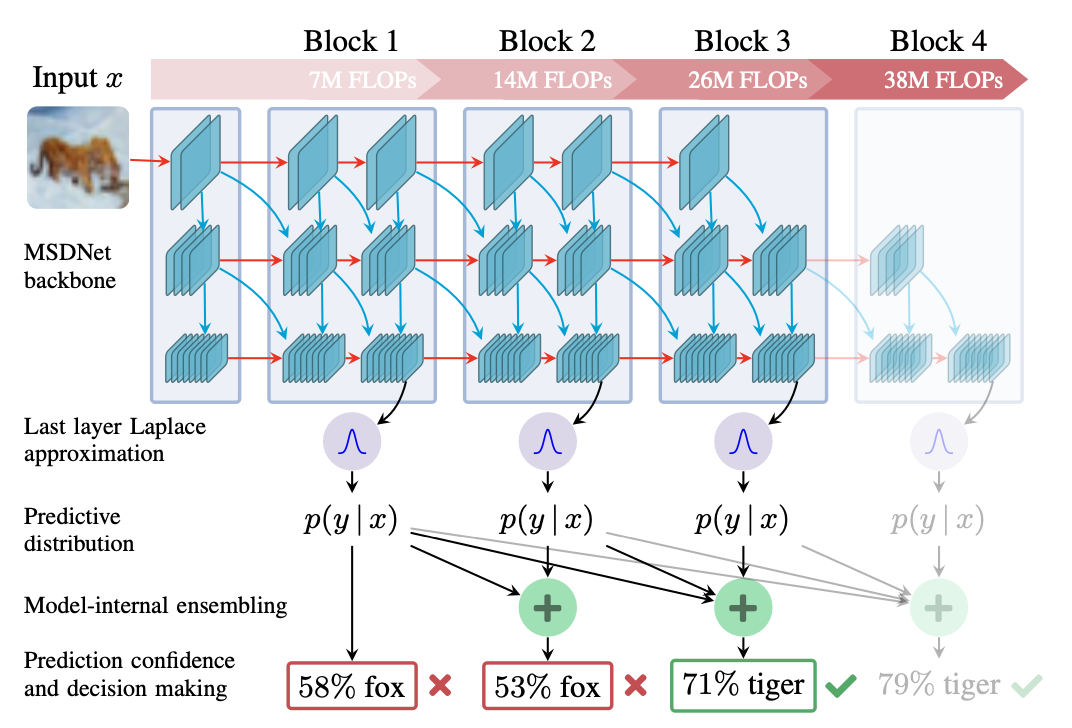
\includegraphics[width=0.4\linewidth]{figs/Screenshot 2025-04-08 at 15.02.28.png}
        \caption{Increasing depth of dynamic neural network}
        \label{fig:enter-label}
    \end{figure}
\end{frame}

\begin{frame}{Background}

    \begin{itemize}
        \item Investigates image classification under budget restrictions \\
              \(\mathcal{D}_{\text{train}} = \left\{ (\mathbf{x}_i, \mathbf{y}_i) \right\}_{i=1}^{n_{\text{train}}}\)
        \item Budget B (FLOPs) must be distributed across a batch for highest possible accuracy
        \item With $n_{block}$ intermediate classifiers, the predictive distribution: \\
              \( p_k(\hat{\mathbf{y}}_i \mid \mathbf{x}_i),\; k = 1, 2, \ldots, n_{\text{block}} \)
        \item Feature representation on the last linear layer \\
              \( \phi_{i,k} = f_k(\mathbf{x}_i) \) with parameters \( \theta_k = \{ \mathbf{W}_k, \mathbf{b}_k \} \)
        \item Prediction of layer k: \\
              \( p_k(\hat{\mathbf{y}}_i \mid \mathbf{x}_i) = \text{softmax}(\hat{\mathbf{z}}_{i,k}), \text{ where } \hat{\mathbf{z}}_{i,k} = \mathbf{W}_k \boldsymbol{\phi}_{i,k} + \mathbf{b}_k \)

    \end{itemize}

\end{frame}

\begin{frame}{Aleatoric and epistemic uncertainty}
    \begin{itemize}
        \item Aleatoric uncertainty is related to randomness intrinsic to the task at hand and cannot be reduced.
        \item Epistemic uncertainty is related to our knowledge of the task and can be reduced by learning more about the task → more data
    \end{itemize}
    \begin{figure}
        \centering
        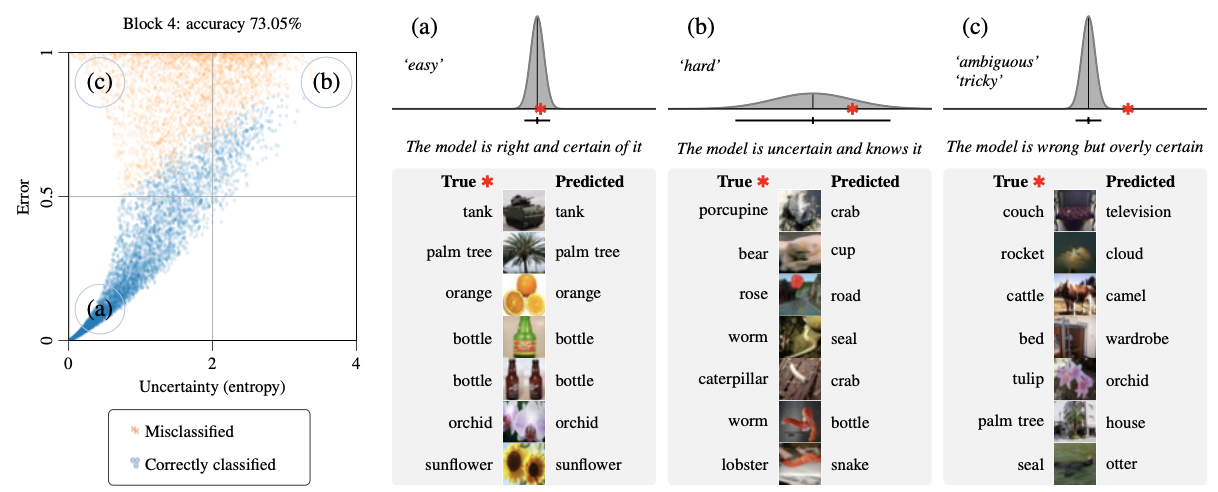
\includegraphics[width=0.7\linewidth]{figs/Screenshot 2025-04-08 at 15.14.46.png}
        \label{fig:enter-label}
    \end{figure}
\end{frame}

\begin{frame}{Bayesian treatment of parameters}
    \[
        p(\boldsymbol{\theta} \mid \mathcal{D}_{\text{train}})
        = \frac{p(\mathcal{D}_{\text{train}} \mid \boldsymbol{\theta}) \, p(\boldsymbol{\theta})}{\int_{\boldsymbol{\theta}} p(\mathcal{D}_{\text{train}}, \boldsymbol{\theta}) \, d\boldsymbol{\theta}}
        = \frac{\text{[likelihood]} \times \text{[prior]}}{\text{[model evidence]}}
    \]


    \begin{itemize}
        \item Posterior distribution over the model parameters is intractable in deep learning
        \item Laplace approximation (second order Taylor expansion)
        \item MAP estimate can be found by maximising the unnormalised posterior:

              \[
                  \hat{\boldsymbol{\theta}} = \arg\max_{\boldsymbol{\theta}} \log p(\mathcal{D}_{\text{train}} \mid \boldsymbol{\theta}) + \log p(\boldsymbol{\theta})
              \]

              \[
                  p(\boldsymbol{\theta} \mid \mathcal{D}_{\text{train}}) \approx \mathcal{N}(\hat{\boldsymbol{\theta}}, \mathbf{H}^{-1})
              \]
    \end{itemize}
    \begin{figure}
        \centering
        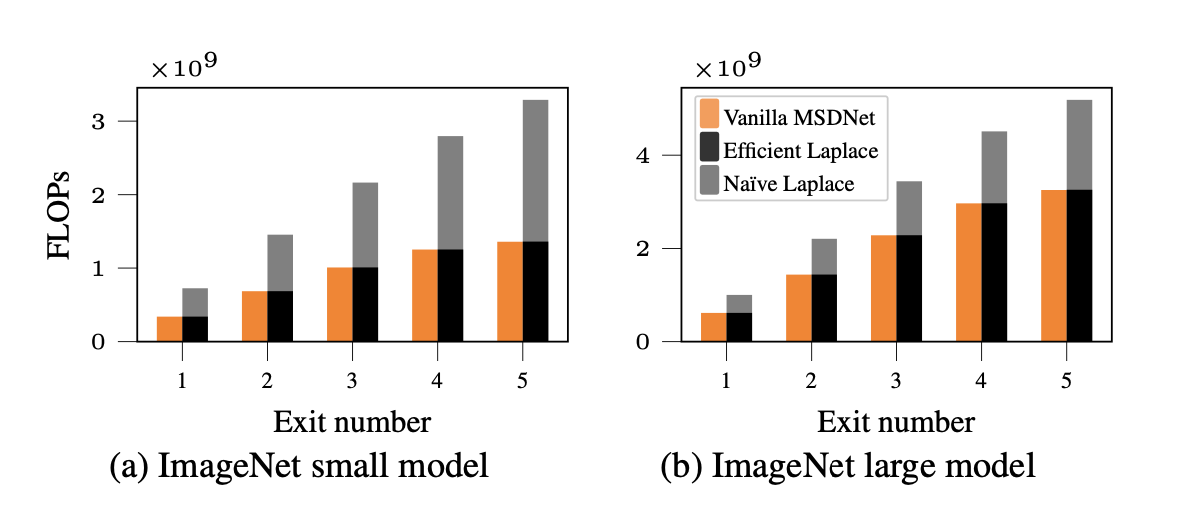
\includegraphics[width=0.5\linewidth]{figs/Screenshot 2025-04-08 at 15.18.50.png}
        \label{fig:enter-label}
    \end{figure}
\end{frame}

\begin{frame}{Method}
    \scriptsize
    \begin{itemize}
        \item Last layer Laplace approximation for each intermediate classifier of the DNN

        \item Final prediction:
              \[
                  \hat{\mathbf{y}}_i = \frac{1}{n_{\text{MC}}} \sum_{l=1}^{n_{\text{MC}}} \text{softmax}(\hat{\mathbf{z}}_i^{(l)})
              \]

        \item Laplace implementation has cost:
              \[
                  {\text{FLOPs}_{\text{efficient}}} = 2c n_{\text{MC}} + 2p^2 + 5p + 2
              \]
              {\footnotesize \quad ($c$: number of classes, $p$: feature dimensionality, $n$: number of MC samples)}

        \item Gaussian distribution:
              \[
                  p(\hat{\mathbf{z}}_i \mid \mathbf{x}_i) = \mathcal{N}(\hat{\mathbf{W}}_{\text{MAP}}^\top \hat{\boldsymbol{\phi}}_i, \, (\hat{\boldsymbol{\phi}}_i^\top \mathbf{V} \hat{\boldsymbol{\phi}}_i) \mathbf{U})
              \]
              \[
                  \mathbf{V}^{-1} \otimes \mathbf{U}^{-1} = \mathbf{H}^{-1}
              \]

        \item Samples:
              \[
                  \hat{\mathbf{z}}_i^{(l)} = \hat{\mathbf{W}}_{\text{MAP}}^\top \hat{\boldsymbol{\phi}}_i + (\hat{\boldsymbol{\phi}}_i^\top \mathbf{V} \hat{\boldsymbol{\phi}}_i)^{\frac{1}{2}} (\mathbf{L} \mathbf{g}^{(l)})
              \]
              {\footnotesize \quad $\mathbf{g}^{(l)} \sim \mathcal{N}(0, \mathbf{I})$ and $\mathbf{L}$ is the Cholesky factor of $\mathbf{U}$}

        \item Temperature scaling is recommended for well-calibrated predictions
    \end{itemize}
\end{frame}

\begin{frame}{Uncertainty}
    \begin{itemize}
        \item The uncertainty should be high for the model to be able to recognize these samples as ‘tricky’, and continue their evaluation to the next block.
        \item For paper model these samples have a high uncertainty, while the vanilla MSDNet is overconfident.
    \end{itemize}
    \begin{figure}
        \centering
        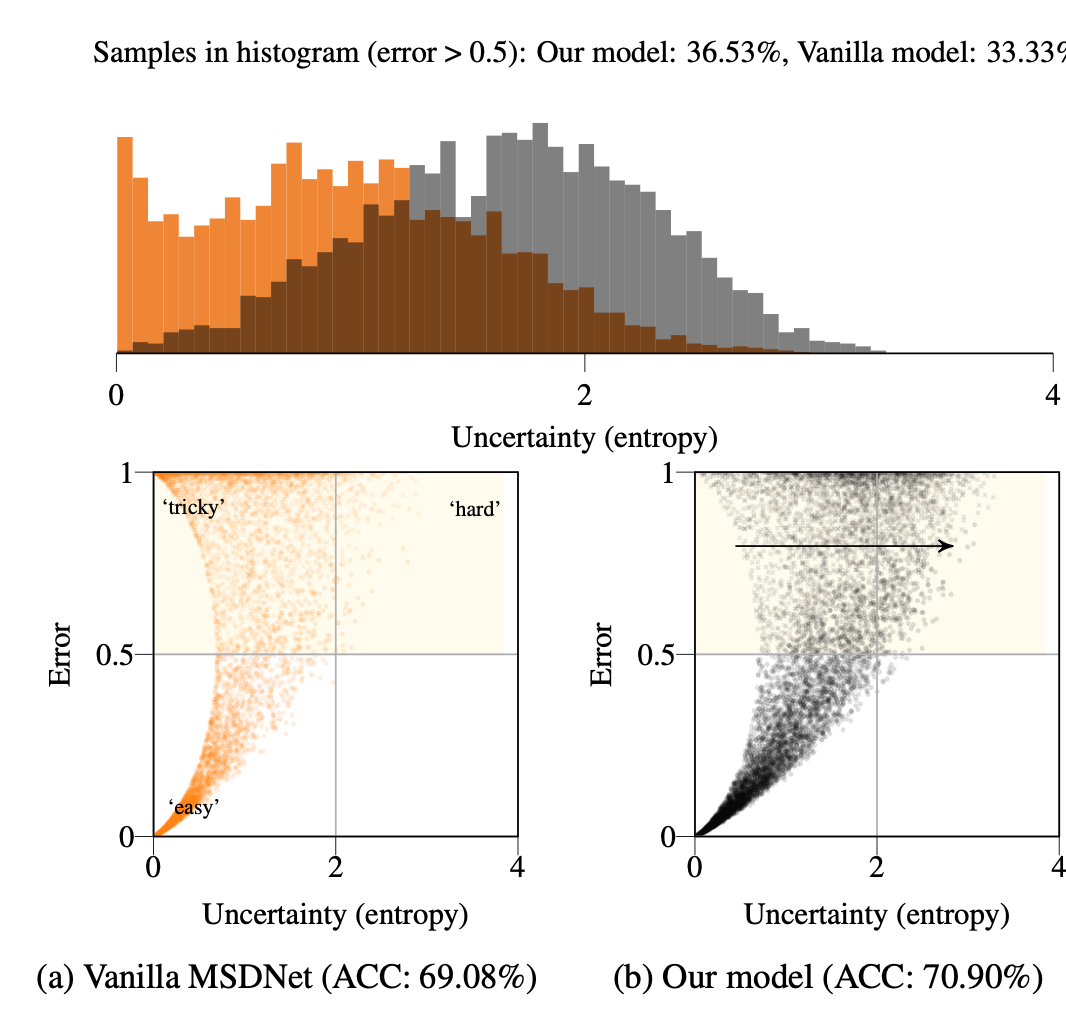
\includegraphics[width=0.35\linewidth]{figs/Screenshot 2025-04-08 at 15.25.23.png}
        \label{fig:enter-label}
    \end{figure}
\end{frame}

\begin{frame}{Ensamble prediction}
    \[
        p_k^{\text{ens}}(\hat{\mathbf{y}}_i \mid \mathbf{x}_i) =
        \frac{1}{\sum_{l=1}^{k} w_l} \sum_{m=1}^{k} w_m \, p_m(\hat{\mathbf{y}}_i \mid \mathbf{x}_i)
    \]

    \vspace{1mm}
    Weights \( w \) are the computational costs in FLOPs up to classifier \( m \)

    \vspace{3mm}
    \begin{itemize}
        \item Early exiting decisions based on model predicted confidence (referred to as MIE)
        \item Thresholds for exiting are calculated on the validation set. Different for every layer (not included in paper)
    \end{itemize}

\end{frame}

\begin{frame}{Results}

    \begin{figure}
        \centering
        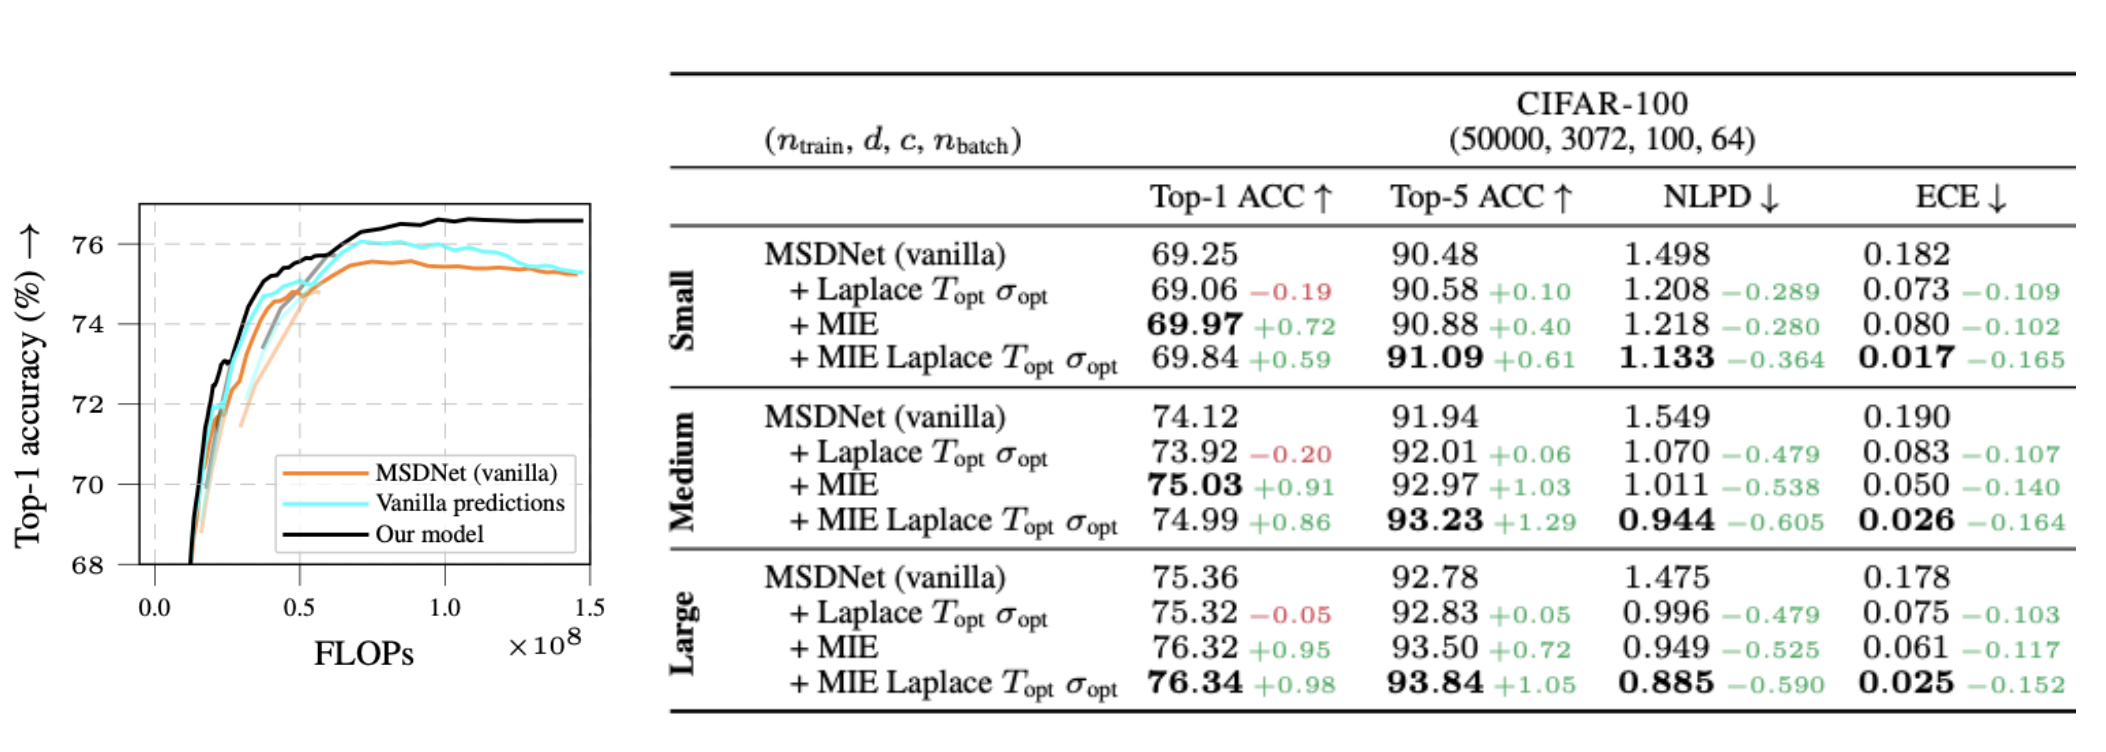
\includegraphics[width=0.8\linewidth]{figs/Screenshot 2025-04-08 at 15.40.28.png}
        \caption{Enter Caption}
        \label{fig:enter-label}
    \end{figure}
    \begin{itemize}
        \item Improving confidence margins in teacher model makes for more efficient knowledge transfer in early exit training
        \item Implementing confidence margins in student model can increase accuracy

    \end{itemize}
\end{frame}

\begin{frame}{For our use}
    \begin{itemize}
        \item Improving confidence margins in teacher model makes for more efficient knowledge transfer in early exit training
        \item Implementing confidence margins in student model can increase accuracy

    \end{itemize}
\end{frame}
%-----------------------------------------------

\begin{frame}{References}
    \footnotesize
    %  \bibliography{reference.bib}
    \bibliographystyle{apalike}
    \bibliography{optML.bib}
\end{frame}

%------------------------------------------------

\begin{frame}
    \Huge{\centerline{\textbf{Thank You}}}
\end{frame}

%----------------------------------------------------------------------------------------

\end{document}